\documentclass{article}

\date{29 septembre 2024}
\usepackage[nb-sem=3, auteurs={George Ober, Félix Rondeau}]{../kholles}


\begin{document}

\maketitle

\allowdisplaybreaks[4]
\begin{question_kholle}
  [Pour tout $(z_{1}, z_{2})\in \mathbb{C}^{2}$,\begin{propositions}

      \item $\lvert z_{1}+z_{2} \rvert \leqslant \lvert z_{1} \rvert + \lvert z_{2} \rvert$

      \item $\bigg| \lvert z_{1} \rvert-\lvert z_{2} \rvert \bigg|\leqslant \lvert z_{1}-z_{2} \rvert$

    \end{propositions}]
  {Preuve de l'inégalité triangulaire et de l'inégalité montrant que le module est 1-lipschitzien + dessin et interprétation géométrique}
  Soient $(z_1,z_2) \in \C^2$ fixés quelconques.
  \begin{itemize}[label=$\lozenge$]
    \item

          Si $z_{2} = 0$ l'inégalité est évidente.\\
          Sinon, $z_{2} \neq 0$ alors $\lvert z_{1}+z_{2} \rvert \leqslant \lvert z_{1} \rvert + \lvert z_{2} \rvert \iff \left| 1+\frac{z_{1}}{z_{2}} \right|\leqslant 1 + \left\lvert  \frac{z_{1}}{z_{2}}  \right\rvert$.\\
          Posons $u = \frac{z_{1}}{z_{2}}$
          \begin{align*}
            \lvert 1+u \rvert ^{2} - (1+\lvert u \rvert )^{2} & = (1+u)(\overline{1+u})-(1+2\lvert u \rvert +\lvert u \rvert ^{2})     \\
                                                              & = (1+u)(1+ \overline u) - 1 - 2\lvert u \rvert  - \lvert u \rvert ^{2} \\
                                                              & = u + \overline u -2 \lvert u \rvert                                   \\
                                                              & = 2(\mathrm{Re}(u)-u) \leqslant 0
          \end{align*}

    \item Appliquons l'inégalité triangulaire
          $$
            \lvert  z_{1} \rvert  = \lvert z_{1} - z_{2} + z_{2} \rvert  \leqslant \lvert z_{1}-z_{2} \rvert +\lvert z_{2} \rvert  \implies \lvert z_{1} \rvert - \lvert z_{2} \rvert \leqslant \lvert z_{1}-z_{2} \rvert
          $$
          Puisque $z_{1}$ et $z_{2}$ jouent de rôles symétriques on a aussi
          $$
            \lvert z_{2} \rvert - \lvert z_{1} \rvert \leqslant \lvert z_{2}-z_{1} \rvert =\lvert z_{1}-z_{2} \rvert
          $$
          Donc
          $$
            \bigg| \lvert z_{1} \rvert-\lvert z_{2} \rvert \bigg|\leqslant \lvert z_{1}-z_{2} \rvert
          $$
          \begin{figure}[H]
            \centering
            \begin{tikzpicture}
              \draw [->] (-0.5,0) -- (10,0);
              \draw [->] (0,-0.5) -- (0,4);
              \draw [-Stealth][line width=1.5] (0,0) -- (10,4) node[midway, above left] {$z_1+z_2$};
              \draw [-Stealth][color=purple,line width=1.5] (0,0) -- (7,1) node[midway, above left] {$z_1$};
              \draw [-Stealth][color=teal,line width=1.5] (7,1) -- (10,4) node[midway, below right] {$z_2$};
            \end{tikzpicture}
            \caption{Interprétation géométrique de l'inégalité triangulaire.}
          \end{figure}
  \end{itemize}

\end{question_kholle}
\begin{question_kholle}{Caractérisation du cas d'égalité de l'inégalité triangulaire dans $\mathbb C$}
  \;\\
  \begin{itemize}[label=$\star$]
    \item ($\implies$) Supposons qu'il y ait égalité dans l'inégalité triangulaire
          \begin{itemize}[label=$\lozenge$]
            \item Si $z_{2} = 0$ alors $z_{1}$ et $z_{2}$ sont positivement liés
            \item Sinon, $\lvert 1+u \rvert ^{2} - (1+\lvert u \rvert )^{2}  = 0$ donc $\mathrm{Re}(u) - \lvert u \rvert = 0$.\\
                  Donc $u \in \mathbb{R}_{+}$, et comme $z_{1} = uz_{2}$, alors $z_{1}$ et $z_{2}$ sont positivement liés.
          \end{itemize}
    \item ($\impliedby$) Supposons que $z_{1}$ et $z_{2}$ sont positivement liés. Alors il existe $\lambda \in \mathbb{R}_{+}$ tel que $z_{1} = \lambda z_{2}$.
          Si $z_{1} = \lambda z_{2}$,
          $$
            \lvert z_{1}+z_{2} \rvert  = \lvert (\lambda+1) z_{2} \rvert  = \lvert \lambda + 1  \rvert \lvert z_{2} \rvert = (\lambda+1)\lvert z_{2} \rvert = \lambda \lvert z_{2} \rvert +\lvert z_{2} \rvert  = \lvert \lambda z_{2} \rvert +\lvert z_{2} \rvert = \lvert z_{1} \rvert + \lvert z_{2} \rvert
          $$
          Donc l'inégalité est une égalité.

          Si $z_{2} = \lambda z_{1}$, en échangeant les rôles joués par $z_{1}$ et $z_{2}$ on obtient que l'inégalité est une égalité.
  \end{itemize}
\end{question_kholle}
\begin{question_kholle}{Calcul de $\sum_{k=0}^{n}\cos(k\theta)$ pour tout $\theta \in \mathbb R$}
  Soit $\theta \in \mathbb{R}$ fixé quelconque, $n \in \mathbb{N}$ fixé quelconque.


  \begin{align*}
    C_{n}(\theta)=\sum_{k=0}^{n} \cos(k\theta) & = \sum_{k=0}^{n} \mathrm{Re}(e^{i k \theta})                                                      \\
                                               & = \mathrm{Re} \left(\sum_{k=0}^{n} e^{i k \theta}\right)                                          \\
                                               & = \mathrm{Re} \left( \sum_{k=0}^{n} (e^{i \theta})^{k} \right) \text{ par les formules de moivre} \\
  \end{align*}
  Ainsi, si $e^{i\theta} = 1 \iff \theta \equiv 0 [2\pi]$,
  $$
    C_{n}(\theta) = \mathrm{Re}\left( \sum_{k=0}^{n}(1)^{k} \right) = \mathrm{Re}(n+1) = n+1
  $$
  Sinon,
  $$
    C_{n}(\theta) = \mathrm{Re}\left( \frac{1-(e^{i\theta})^{n+1}}{1-e^{i\theta}} \right)
  $$
  Simplifions donc ce quotient.

  \begin{align*}
    \frac{1-(e^{i\theta})^{n+1}}{1-e^{i\theta}} = \frac{1-e^{i\theta(n+1)}}{1-e^{i\theta}}
     & =\frac{e^{\frac{i\theta(n+1)}2{}}\left( e^{-\frac{i\theta(n+1)}2{}}-e^{\frac{i\theta(n+1)}2{}} \right)}{e^{i\frac{\theta}{2}}\left( e^{-i\frac{\theta}{2}}- e^{i \frac{\theta}{2}} \right)} \\
     & = e^{i \frac{\theta n}2}\left( \frac{-2i \sin\left( \frac{\theta (n+1)}{2} \right)}{-2i\sin \frac{\theta}{2}} \right)                                                                       \\
     & = \frac{\sin\left( \frac{\theta(n+1)}{2} \right)}{\sin \frac{\theta}{2}}\left( \cos \frac{\theta n}{2} + i \sin \frac{\theta n}{2} \right) \tag{$\clubsuit$}\label{S3:Q3}
  \end{align*}


  En prenant la partie réelle de ce résultat, on a
  $$
    C_{n}(\theta) = \mathrm{Re}\left[ \frac{\sin\left( \frac{\theta(n+1)}{2} \right)}{\sin \frac{\theta}{2}}\left( \cos \frac{\theta n}{2} + i \sin \frac{\theta n}{2} \right) \right] = \frac{\sin\left( \frac{\theta(n+1)}{2} \right)}{\sin \frac{\theta}{2}} \cos \frac{n\theta}{2}
  $$

  Donc
  $$
    C_{n}(\theta) = \left\{ \begin{array}{ll}
      n+1                                                                                           & \text{ si } \theta \equiv 0 [2 \pi] \\
      \frac{\sin\left( \frac{\theta(n+1)}{2} \right)}{\sin \frac{\theta}{2}} \cos \frac{n\theta}{2} & \text{ sinon}
    \end{array}\right.
  $$
\end{question_kholle}
\textbf{Remarque}
En prenant la partie imaginaire de \eqref{S3:Q3}, on peut retrouver la somme $S_n(\theta)$:
$$
  S_{n}(\theta)= \sum_{k=0}^n \sin(k \theta) = \left\{ \begin{array}{ll}
    0                                                                                             & \text{ si } \theta \equiv 0 [2 \pi] \\
    \frac{\sin\left( \frac{\theta(n+1)}{2} \right)}{\sin \frac{\theta}{2}} \sin \frac{n\theta}{2} & \text{ sinon}
  \end{array}\right.
$$
\begin{question_kholle}
  [{Soient $n \in \mathbb{N}, (a_{0}, \dots, a_{n})\in\mathbb{C}^{n+1}$ et $z_{0} \in \mathbb{C}$ Posons pour tout $z \in \mathbb{C}, P(z) = \sum_{k=0}^{n}a_{k}z^{k}$
  \begin{propositions}
    \item Si $P(z_{0}) = 0$, alors $\exists Q \in\mathbb{C}[z]:\forall z \in \mathbb{C}, P(z)=(z-z_{0})Q(z)$
  \end{propositions}
  }]
  {Si $z_0$ est racine de la fonction polynômiale $P$, alors $P$ se factorise par $(z-z_0)$}
  Soit $z \in \mathbb{C}$ fixé quelconque,
  \begin{align*}
    P(z) & = P(z) - P(z_{0})                                                                                                        \\
         & = \sum_{k=0}^{n}a_{k}z^{k} - \sum_{k=0}^{n}a_{k}z_{0}^{k}                                                                \\
         & = \sum_{k=0}^{n}a_{k}(z^{k}-z_{0}^{k})                                                          & \text{ nul pour }k = 0 \\
         & = \sum_{k=1}^{n}\left( a_{k}(z-z_{0})\left( \sum _{j=0}^{k-1}z^{j}z_{0}^{k-1-j} \right) \right)                          \\
         & = (z-z_{0}) \sum_{k=1}^{n}a_{k}\left( \sum _{j=0}^{k-1}z^{j}z_{0}^{k-1-j} \right)
  \end{align*}

  Donc en posant $Q(z) = \sum_{k=1}^{n}a_{k}\left( \sum _{j=0}^{k-1}z^{j}z_{0}^{k-1-j} \right), \in \mathbb{C}[z]$, on a montré que $P$ se factorise.
\end{question_kholle}
\begin{question_kholle}{Si $z_1, \dots , z_n$ sont $n$ racines distinctes de la fonction polynômiale $P$ de degré $n$, alors $P(z)$ se factorise en ... }
  Soient $n\in\N$ et $(a_0,\dots,a_n)\in\C^n\times\C^*$ fixés quelconques. Posons, pour tout $z\in\C$,
  \begin{align}\label{eqn:S3:5.1}
    P(z)=\sum_{k=0}^{n}{a_kz^k}
  \end{align}
  Supposons que $(z_1,\dots,z_n)\in\C^n$ sont $n$ racines deux à deux distinctes de la fonction polynomiale $P$. Alors, il existe $Q\in\C[z]$ tel que pour tout $z\in\C$,
  \begin{align*}
    P(z)=Q(z)\prod_{i=1}^{n}{(z-z_i)}
  \end{align*}
  On note $d$ le degré de $Q$ et $(b_0, b_d)\in\C^d\times\C^*$ ses coefficients. On a alors
  \begin{align*}
    Q(z)=\sum_{k=0}^{d}{b_dz^d}
  \end{align*}
  Ainsi, $P(z)$ s'écrit
  \begin{align}\label{eqn:S3:5.2}
    P(z)=\sum_{k=0}^{d}{b_dz^d}\prod_{i=1}^{n}{(z-z_i)} = b_dz^{n+d} + \textit{termes de degré inférieur à $n+d$.}
  \end{align}
  Par unicité des coefficients d'une fonction polynomiale, $n+d=n$ (sinon, $z^{n+d}$ aurait un coefficient $b_d$ non nul à droite mais un coefficient nul à gauche).\\
  Donc $d=0$ d'où $Q$ est une fonction constante de valeur $b_d=b_0$, et en identifiant les termes en $z^n$ de \eqref{eqn:S3:5.1} et \eqref{eqn:S3:5.2}, on obtient $a_n=b_0$. Ainsi, pour tout $z\in\C$,
  \begin{align*}
    P(z)=a_n\prod_{i=1}^{n}{(z-z_i)}
  \end{align*}
\end{question_kholle}
\begin{question_kholle}{Calculer le module et un argument de $z=1+ e^{i \theta}$ en fonction de $\theta \in [0, 2 \pi[$}
  Soit $\theta \in [0, 2\pi[$
  $$
    z = 1+ e^{i \theta} = e^{i\times0}+e^{i\theta} = e^{i \frac{\theta}{2}}\left( e^{-i\frac{\theta}{2}} + e^{i \frac{\theta}{2}} \right)= 2 \cos \frac{\theta}{2}e^{i\frac{\theta}{2}}
  $$
  Cette dernière notation est une notation exponentielle seulement si $2 \cos \frac{\theta}{2} \geqslant 0$.
  \begin{itemize}[label=$\star$]
    \item Si $\theta \in [0, \pi[$,
          $$\left\{ \begin{array}{ll}
              |z| = 2\cos \frac{\theta}{2} \\
              \frac{\theta}{2} \in \mathrm{Arg}  (z)
            \end{array}\right.$$
    \item Si $\theta = \pi$, $z = 0$ donc $\lvert z \rvert = 0$

    \item Si $\theta \in ]\pi, 2\pi[$,

          \begin{align*}
            z = 2 \cos \frac{\theta}{2}e^{i\frac{\theta}{2}} & = -2 \left\lvert  \cos \frac{\theta}{2}  \right\rvert e^{i\frac{\theta}{2}}                      \\
                                                             & =-2 \left\lvert  \cos \frac{\theta}{2}  \right\rvert e^{i \left( \frac{\theta}{2} + \pi \right)}
          \end{align*}

          Donc
          $$
            \left\{ \begin{array}{ll}
              |z| = -2 \lvert  \cos \frac{\theta}{2}  \rvert \\
              \frac{\theta}{2} + \pi \in \mathrm{Arg}  (z)
            \end{array}\right.
          $$
  \end{itemize}
\end{question_kholle}
\begin{question_kholle}[{Considérons l'équation algébrique de degré 2:
        $$az^{2}+bz+c=0$$
        Où $z\in L$ est l'inconnue et $(a,b,c)\in\mathbb{C}^*\times\mathbb{C}^2$ sont des paramètres. Posons $\Delta = b^{2}-4ac$ que l'on appelle le discriminant de l'équation.
        \begin{itemize}
          \item Si $\Delta=0$, l'équation admet une unique solution dite double qui est $-\frac b{2a}$ et la forme factorisée du trinôme est
                $$
                  az^2+bz+c = a \left( z + \frac b {2a} \right)^2
                $$
          \item Si $\Delta\neq0$, notons $\delta$ une racine carrée de $\Delta$, l'équation admet deux solutions distinctes $\frac{-b-\delta}{2a}$ et $\frac{-b+\delta}{2a}$ dites simples et la forme factorisée du trinôme est
                $$
                  az^2+bz+c = a\left(z - \frac{-b-\delta}{2a}\right)\left(z - \frac{-b+\delta}{2a}\right)
                $$
        \end{itemize}
      }]{Résolution des équations algébriques de degré $2$ dans $\C$ et algorithme de recherche d'une racine carrée sous forme cartésienne (sur un exemple explicite).}
  La preuve est immédiate à partir de la forme canonique du trinôme du second degré :

  La preuve est immédiate à partir de la forme canonique du trinôme du second degré :

  \begin{align*}
    az^{2}+bz+c = a\left[ \underbrace{ z^{2}+\frac{b}{a}z }_{ \text{But: Absorber ces termes dans un carré} }+\frac{c}{a} \right] & = a\left[ z^{2}+2\frac{b}{2a}z +\frac{b^{2}}{4a^{2}}-\frac{b^{2}}{4a^{2}}+\frac{c}{a} \right] \\
                                                                                                                                  & =a \left[ \left( z+\frac{b}{2a} \right)^{2} - \frac{b^{2}}{4a^{2}}+\frac{c}{a} \right]        \\
                                                                                                                                  & =a \left[ \left( z+\frac{b}{2a} \right)^{2} - \frac{b^{2}-4ac}{4a^{2}}\right]                 \\
                                                                                                                                  & =a \left[ \left( z+\frac{b}{2a} \right)^{2} - \frac{\Delta}{4a^{2}}\right]
  \end{align*}
  \begin{itemize}
    \item Si $\Delta = 0$
          $$
            az^{2}+bz+c = a\left( z-\frac{-b}{2a} \right)^{2}
          $$
          de sorte que
          $$
            az^{2}+bz+c = 0 \iff a\left( z-\frac{-b}{2a} \right)^{2} = 0 \iff z = -\frac{b}{2a}
          $$

    \item Sinon
          \begin{align*}
            az^{2}+bz+c = a \left[ \left( z+\frac{b}{2a} \right)^{2}-\left( \frac{\delta}{2a} \right)^{2} \right] & = a \left( z + \frac{b}{2a}-\frac{\delta}{2a} \right)\left( z+\frac{b}{2a}+\frac{\delta}{2a} \right) \\ &= a \left( z - \frac{-z+\delta}{2a} \right)\left( z- \frac{-z - \delta}{2a} \right)
          \end{align*}
          de sorte que

          \begin{align*}
            az^{2}+bz+c =0 & \iff a \left( z - \frac{-z+\delta}{2a} \right)\left( z- \frac{-z - \delta}{2a} \right) = 0 \\ \\
                           & \iff \left\{ \begin{array}{ll}
                                            z -  \frac{-z-\delta}{2a}  = 0 \\
                                            \text{ou}                      \\
                                            z- \frac{-z+\delta}{2a} =0
                                          \end{array}\right.                                                \\
                           & \iff \left\{ \begin{array}{ll}
                                            z = \frac{-z-\delta}{2a} \\ \text{ou} \\
                                            z = \frac{-z+\delta}{2a}
                                          \end{array}\right.
          \end{align*}

  \end{itemize}
\end{question_kholle}

\pagebreak
\begin{question_kholle}[{
  Pour tout $n \in \mathbb N ^{*} \setminus \{ 1 \}$,
  $$
    \mathbb U _n = \left\{ e^{\frac{2ik\pi}{n}}\mid k \in [ \! [ 0, n - 1 ] \!] \right\}
  $$
  }]{Décrire (avec preuve) l'ensemble des racines $n$-ièmes de l'unité et les localiser géométriquement dans le plan complexe.}
  \begin{itemize}
    \item \underline{Description de l'ensemble $\mathbb U _n$}
          \begin{align*}
            \left\{ \begin{array}{ll}
                      z^{n}=1 \\
                      z \in \mathbb{C}
                    \end{array}\right.
             & \iff
            \left\{ \begin{array}{ll}
                      z^{n} = 1 \\
                      z \in \mathbb{C}^{*}
                    \end{array}\right. \text{ ou }
            \left\{ \begin{array}{ll}
                      z^{n} = 1 \\
                      z = 0
                    \end{array}\right.                                               \\
             & \iff
            \left\{ \begin{array}{ll}
                      \rho^{n}e^{in \theta}  = 1 \\
                      z = \rho e^{i \theta}      \\
                      (\rho, \theta) \in \mathbb{R}_{+}^{*}\times \mathbb{R}
                    \end{array}\right.
            \\ & \iff
            \left\{ \begin{array}{ll}
                      \rho^{n} = 1              \\
                      n \theta \equiv 0 [2 \pi] \\
                      z = \rho e^{i \theta}     \\
                      (\rho, \theta) \in \mathbb{R}_{+}^{*}\times \mathbb{R}
                    \end{array}\right.
            \\ & \iff
            \left\{ \begin{array}{ll}
                      \rho = 1 \text{ car } \rho > 0                \\
                      \theta \equiv 0 \left[ \frac{2\pi}{n} \right] \\
                      z = \rho e^{i \theta}                         \\
                      (\rho, \theta) \in \mathbb{R}_{+}^{*}\times \mathbb{R}
                    \end{array}\right.
            \\ & \iff
            \left\{ \begin{array}{ll}
                      \rho = 1                                            \\
                      \exists k \in \mathbb{Z} : \theta = \frac{2k\pi}{n} \\
                      z = \rho e^{i \theta}                               \\
                      (\rho, \theta) \in \mathbb{R}_{+}^{*}\times \mathbb{R}
                    \end{array}\right.
            \\  & \iff \exists k \in \mathbb{Z}: z=e^{\frac{2ik\pi}{n}} \\
             & \iff z \in \left\{ e^{\frac{2ik\pi}{n}}\mid k \in \mathbb{Z} \right\}
          \end{align*}


          L'ensemble des solutions est paramétré par l'entier $k$ qui parcourt un ensemble infini. Toutefois, en représentant graphiquement les solutions, il semblerait que "tous les $n$", on fait un tour de cercle trigonométrique de plus, en redécrivant les solutions déjà obtenues pour $k \in [ \! [ 0, n-1 ] \!]$.
    \item \underline{Localisation géométrique}
          \begin{itemize}[label=$\star$]
            \item $\mathbb U _3$ est l'ensemble des sommets du triangle équilatéral inscrit dans le cercle unité, et dont $1$ est l'un des sommets

            \item $\mathbb U _4$ est l'ensemble des sommets du carré inscrit dans le cercle unité et dont 1 est l'un des sommets. Le côté du carré vaut $\lvert 1 - i\rvert = \sqrt 2$.
            \item $\mathbb U _5$ est l'ensemble des sommets du pentagone régulier inscrit dans le cercle unité et dont 1 est l'un des sommets.
                  \begin{figure}[!h]
                    \hfill
                    \begin{minipage}{.45\textwidth}
                      \centering
                      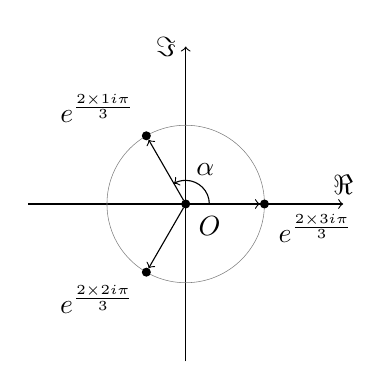
\begin{tikzpicture}[
                          dot/.style={draw,fill,circle,inner sep=1pt}
                        ]
                        \draw[->] (-2,0) -- (2,0) node[above] {$\Re$};
                        \draw[->] (0,-2) -- (0,2) node[left] {$\Im$};
                        \draw[help lines] (0,0) circle (1);

                        \node[dot,label={below right:$O$}] (O) at (0,0) {};
                        \foreach \i in {1,...,3} {
                            \node[dot,label={\i*360/3-(\i==3)*45:$e^\frac{2 \times {\i} i \pi}{3}$}] (w\i) at (\i*360/3:1) {};
                            \draw[->] (O) -- (w\i);
                          }
                        \draw[->] (0:.3) arc (0:360/3:.3);
                        \node at (360/3/2:.5) {$\alpha$};
                      \end{tikzpicture}
                      \caption{Racines cubiques de l'unité.}
                    \end{minipage}
                    \begin{minipage}{.45\textwidth}
                      \centering
                      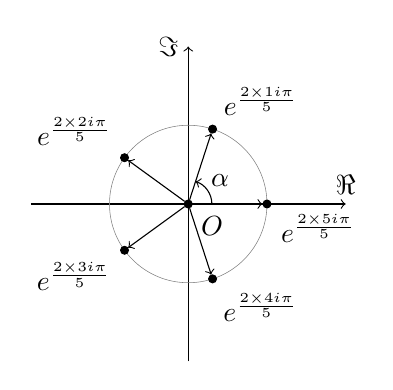
\begin{tikzpicture}[
                          dot/.style={draw,fill,circle,inner sep=1pt}
                        ]
                        \draw[->] (-2,0) -- (2,0) node[above] {$\Re$};
                        \draw[->] (0,-2) -- (0,2) node[left] {$\Im$};
                        \draw[help lines] (0,0) circle (1);

                        \node[dot,label={below right:$O$}] (O) at (0,0) {};
                        \foreach \i in {1,...,5} {
                            \node[dot,label={\i*360/5-(\i==5)*45:$e^\frac{2 \times {\i} i \pi}{5}$}] (w\i) at (\i*360/5:1) {};
                            \draw[->] (O) -- (w\i);
                          }
                        \draw[->] (0:.3) arc (0:360/5:.3);
                        \node at (360/5/2:.5) {$\alpha$};
                      \end{tikzpicture}
                      \caption{Racines $5^{\mathrm{èmes}}$ de l'unité.}
                    \end{minipage}
                  \end{figure}
          \end{itemize}
  \end{itemize}
\end{question_kholle}
\pagebreak
\begin{question_kholle}{Somme et Produit des racines $n$-ièmes}
  \;\\
  \begin{itemize}[label=$\lozenge$]
    \item \textbf{Méthode 1} : En utilisant les relations coefficients racines.

          $\mathbb{U}_{n}$ sont les n racines disctinctes de $z^{n}-1$
          $$S_{n} = - \frac{1}{\text{coefficient dominant}}\times(\text{coefficient de }z^{n-1} \text{ dans }z^{n}-1)= \left\{ \begin{array}{ll}
              -0    & \text{ si }  n\geqslant 2 \\
              -(-1) & \text{ sinon}
            \end{array}\right.$$
          $$
            P_{n} = (-1)^{n} \frac{\text{coefficient constant}}{\text{coefficient dominant}} = (-1) ^{n}\times \frac{-1}{1} = (-1)^{n+1}
          $$

    \item \textbf{Méthode 2} : Manipulation des symboles sommatoires

          \begin{align*}
            S_{n} = \sum_{\omega \in \mathbb{U}_{n}}\omega & = \sum_{k=0}^{n-1}\omega_{0}^{k}                                                                    \\
                                                           & = \left\{ \begin{array}{ll}
                                                                         1                                                & \text{si }  n =1 \\
                                                                         1 \times \frac{1 - \omega_{0}^{n}}{1-\omega_{0}} & \text{sinon}
                                                                       \end{array}\right.
          \end{align*}

          Puisqu'on ne peut appliquer la formule de la somme des termes d'une suite géométrique seulement si $\omega_{0} = 1 \iff e^{\frac{2i\pi}{n}} = 1 \iff \frac{2\pi}{n} \equiv 0 [2\pi] \iff n = 1$

          De même

          \begin{align*}
            P_{n} = \prod_{\omega \in \mathbb{U}_{n}}\omega = \prod_{k=0}^{n-1}\omega_{0}^{k}= \omega_{0}^{\sum_{k=0}^{n-1}k} & = \omega_{0} ^{\frac{n(n-1)}{2}}                                                                                  \\ \\
                                                                                                                              & =\left\{ \begin{array}{ll}
                                                                                                                                           (\omega_{0}^{n})^{\frac{n-1}{2}} = 1^{\frac{n-1}{2}} = 1 & \text{si } n \equiv 1 [2] \\
                                                                                                                                           e^{\frac{2i\pi n(n-1)}{2n}} = e^{i \pi(n-1)} = (-1)^{n-1}
                                                                                                                                         \end{array}\right.
            \\ &= (-1)^{n-1}
          \end{align*}
  \end{itemize}
\end{question_kholle}
\begin{question_kholle}
  [{Soient $n \in \mathbb{N}, (a_{0}, \dots, a_{n})\in\mathbb{C}^{n+1}$ et $z_{0} \in \mathbb{C}$.\\
  Posons pour tout $z \in \mathbb{C}, P(z) = \sum_{k=0}^{n}a_{k}z^{k}$.
  \begin{propositions}
    \item Si $\exists p \in \mathbb{N}^{*}: \exists(z_{1},\dots ,z_{p})\in\mathbb{C}^{p}$ deux à deux distincts tels que $\forall k \in [ \! [ 1, p ] \!], P(z_{k}) = 0$ alors, $\exists Q \in \mathbb{C}[x]:\forall z \in \mathbb{C}, P(z) = Q(z) \times \prod_{k=1}^{p}(z-z_{k})$.
  \end{propositions}
  }]
  {\textit{[non demandée]} Factorisation d'une fonction polynomiale connaissant $p$ racines.}
  Considérons la propriété $\mathcal{P}(\cdot)$ définie pour tout $p \in \mathbb{N}^{*}$ par
  \begin{multline*}
    \mathcal{P}(p) : \forall P \in \mathbb{C}[z], (\exists (z_{1}, \dots, z_{p}) \in \mathbb{C}^{p}, \text{ 2 à 2 distincts }: \forall i \in [ \! [ 1, p ] \!], P(z_{i}) = 0)\\
    \implies \exists Q \in \mathbb{C}[z]: P(z) = Q(z) \prod_{i=1}^{p}(z-z_{i})
  \end{multline*}
  \begin{itemize}[label=$\lozenge$]
    \item $\mathcal{P}(1)$ est vraie d'après la preuve précédente.
    \item Soit $p \in \mathbb{N}^{*}$ fixé quelconque tel que $\mathcal{P}(p)$ est vraie.\\
          Soit $P \in \mathbb{C}[z]$ fixés quelconques tels que $\exists (z_{1}, \dots, z_{p+1}) \in \mathbb{C} ^{p+1}$ deux à deux distincts tels que $\forall i \in [ \! [ 1, p + 1 ] \!], P(z_{i}) = 0$.\\
          Appliquons $\mathcal{P}(p)$ à $P \in \mathbb{C}[z]$ dont $(z_{1}, \dots, z_{p})$ sont les $p$ racines deux à deux distinctes.

          $$\exists Q_{1} \in \mathbb{C}[z]:\forall z \in \mathbb{C}, P(z) = Q_{1}(z)\prod_{i=1}^{p}(z-z_{i})$$
          Évaluons cette expression en $z_{p+1}$
          $$\underbrace{ P(z_{p+1}) }_{ =0 } = Q_{1}(z_{p+1}) \prod_{i=1}^{p}\underbrace{ (z_{p+1}-z_{i}) }_{ \neq 0 \text{ car distincts} }$$
          Donc $Q_{1}(z_{p+1}) = 0$, ce qui permet d'appliquer (i) pour $P \leftarrow Q_{1}$, $z_{0} \leftarrow z_{p+1}$.
          $$
            \exists Q \in \mathbb{C}[z]:\forall z \in \mathbb{C}, Q_{1}(z)=(z-z_{p+1})Q(z)
          $$
          Donc
          $$
            \forall z \in \mathbb{C}, P(z) = (z-z_{p+1})Q(z) \prod_{i=1}^{p}(z-z_{i}) = Q(z) \prod_{i=1}^{p+1}(z-z_{i})
          $$
          Donc $\mathcal{P}(p+1)$ est vraie.
  \end{itemize}
\end{question_kholle}
\end{document}
